\documentclass{article}\usepackage[]{graphicx}\usepackage[]{color}
%% maxwidth is the original width if it is less than linewidth
%% otherwise use linewidth (to make sure the graphics do not exceed the margin)
\makeatletter
\def\maxwidth{ %
  \ifdim\Gin@nat@width>\linewidth
    \linewidth
  \else
    \Gin@nat@width
  \fi
}
\makeatother

\definecolor{fgcolor}{rgb}{0.345, 0.345, 0.345}
\newcommand{\hlnum}[1]{\textcolor[rgb]{0.686,0.059,0.569}{#1}}%
\newcommand{\hlstr}[1]{\textcolor[rgb]{0.192,0.494,0.8}{#1}}%
\newcommand{\hlcom}[1]{\textcolor[rgb]{0.678,0.584,0.686}{\textit{#1}}}%
\newcommand{\hlopt}[1]{\textcolor[rgb]{0,0,0}{#1}}%
\newcommand{\hlstd}[1]{\textcolor[rgb]{0.345,0.345,0.345}{#1}}%
\newcommand{\hlkwa}[1]{\textcolor[rgb]{0.161,0.373,0.58}{\textbf{#1}}}%
\newcommand{\hlkwb}[1]{\textcolor[rgb]{0.69,0.353,0.396}{#1}}%
\newcommand{\hlkwc}[1]{\textcolor[rgb]{0.333,0.667,0.333}{#1}}%
\newcommand{\hlkwd}[1]{\textcolor[rgb]{0.737,0.353,0.396}{\textbf{#1}}}%

\usepackage{framed}
\makeatletter
\newenvironment{kframe}{%
 \def\at@end@of@kframe{}%
 \ifinner\ifhmode%
  \def\at@end@of@kframe{\end{minipage}}%
  \begin{minipage}{\columnwidth}%
 \fi\fi%
 \def\FrameCommand##1{\hskip\@totalleftmargin \hskip-\fboxsep
 \colorbox{shadecolor}{##1}\hskip-\fboxsep
     % There is no \\@totalrightmargin, so:
     \hskip-\linewidth \hskip-\@totalleftmargin \hskip\columnwidth}%
 \MakeFramed {\advance\hsize-\width
   \@totalleftmargin\z@ \linewidth\hsize
   \@setminipage}}%
 {\par\unskip\endMakeFramed%
 \at@end@of@kframe}
\makeatother

\definecolor{shadecolor}{rgb}{.97, .97, .97}
\definecolor{messagecolor}{rgb}{0, 0, 0}
\definecolor{warningcolor}{rgb}{1, 0, 1}
\definecolor{errorcolor}{rgb}{1, 0, 0}
\newenvironment{knitrout}{}{} % an empty environment to be redefined in TeX

\usepackage{alltt}
\usepackage{fullpage}
\usepackage{placeins}
\usepackage{graphicx}
\usepackage[colorlinks=true,linkcolor=blue]{hyperref}
\title{Lab 4 Spatial Interpolation}
\author{Dominic LaRoche}
\date{October 2, 2014}
\IfFileExists{upquote.sty}{\usepackage{upquote}}{}
\begin{document}
\maketitle

\tableofcontents

\section{Assignment I: Allocation Analysis}
The allocation maps for precipitation, maximum temperature, and minimum temperature are found in figures ~\ref{alloprecip}, ~\ref{allomax}, and~\ref{allomin} respectively.  Since all three of these variables are probably distributed continuously accross the landscape the non-smooth allocation is probably a poor interpolation near the edges of the polygons.\\

\begin{figure}
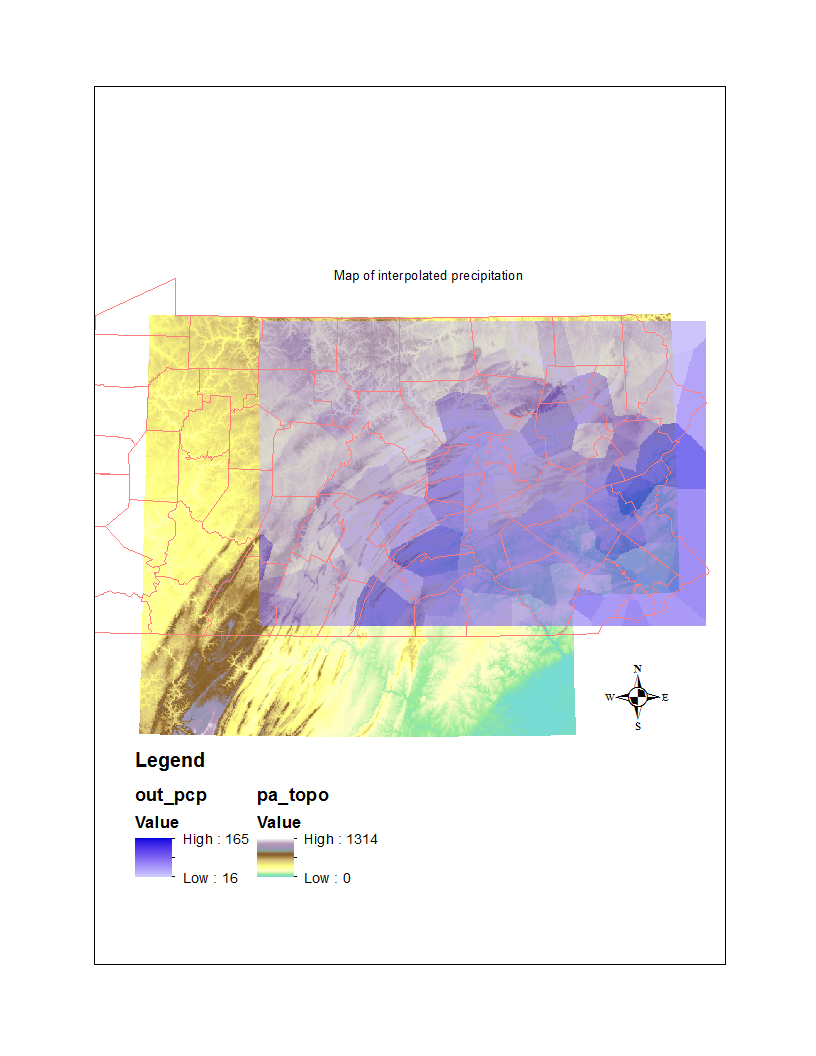
\includegraphics[scale=.9]{./figure/Precip}
\caption{Map of allocation for precipitation}
\label{alloprecip}
\end{figure}

\begin{figure}
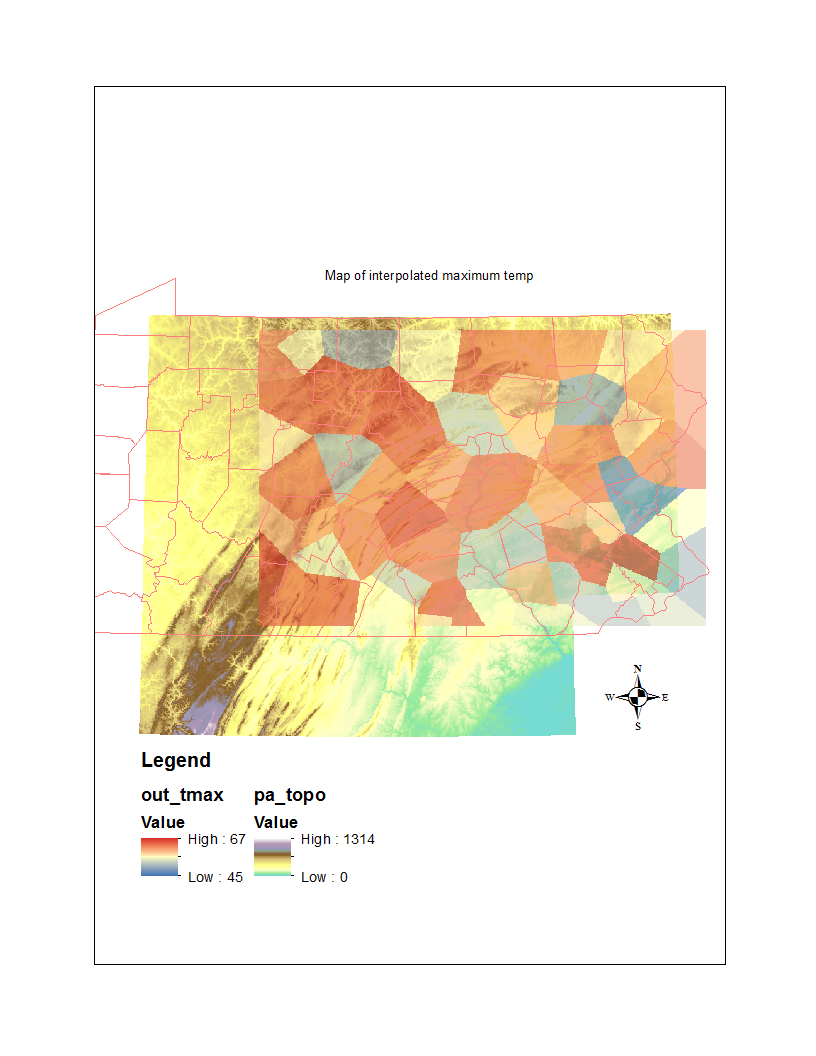
\includegraphics[scale=.9]{./figure/MaxTemp}
\caption{Map of allocation for precipitation}
\label{allomax}
\end{figure}

\begin{figure}
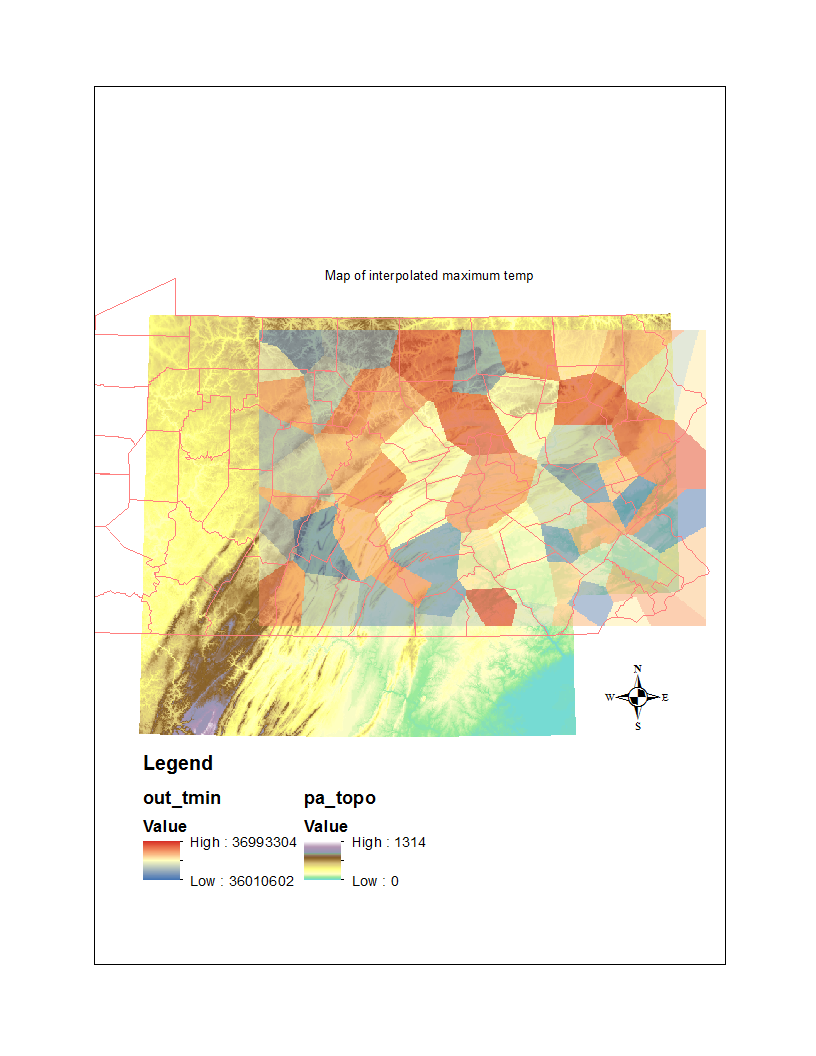
\includegraphics[scale=.9]{./figure/MinTemp}
\caption{Map of allocation for precipitation}
\label{allomin}
\end{figure}


\FloatBarrier

\section{Assignment II: Inverse Distance Weighting}
I used three different powers for the inverse distance weighting, 1, 3, and 4 (figs. ~\ref{IDWprecip1},~\ref{IDWprecip2}, and~\ref{IDWprecip4}).  The best power for precipitation appeared to be 2 (the default).  At small power there appeared to be too much weight immediately adjacent to weather stations and the surface was too rough.  At a power=2 the surface appeared to be smoother and the trend in precipitation was more clearly represented.  Power=4 appeared to create a patchy surface.\\
For temperature power=1 appeared to be the best option I tried, althoug in hindsight I should have tried a fractional power such as .5 since there are still identifiable weather stations with power 1.  However, even with power 1 it is clear that the high elevation areas have both higher max temperatures (~\ref{idwmax1}) and lower min temperatures (\ref{idwmin1}).\\

\begin{figure}
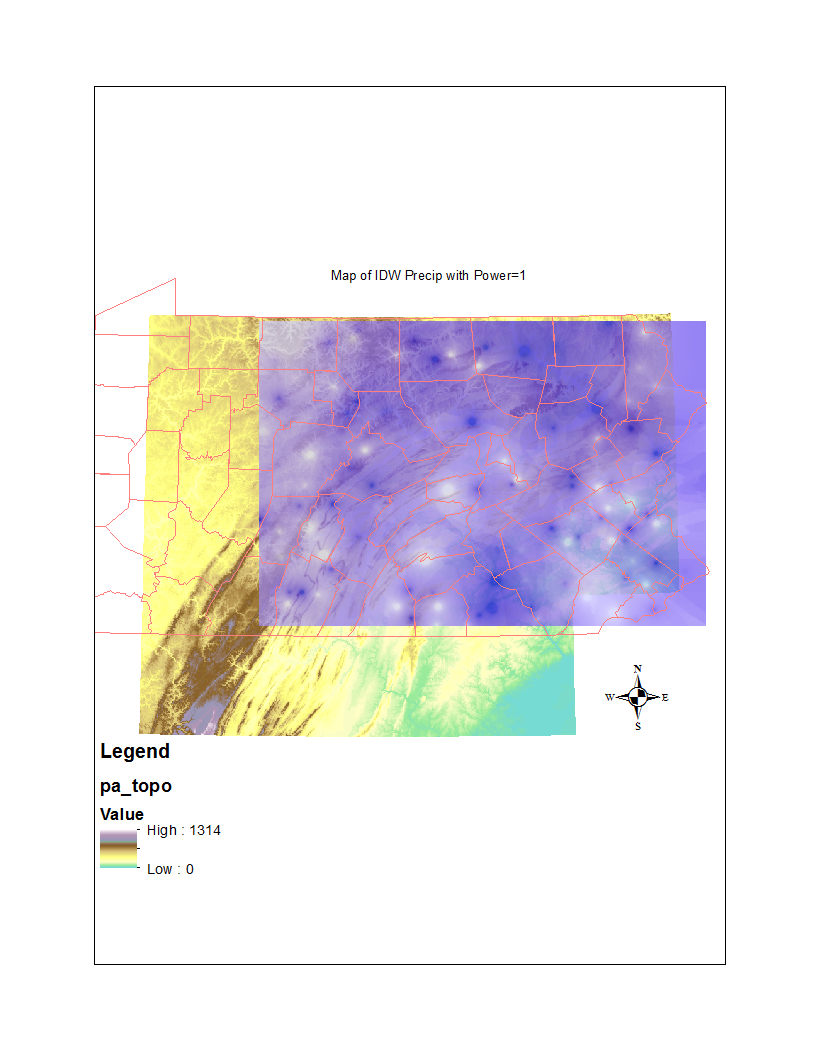
\includegraphics[scale=.9]{./figure/IDWprecip}
\caption{Map of inverse distance weighting for precipitation with power=1.}
\label{IDWprecip1}
\end{figure}

\begin{figure}
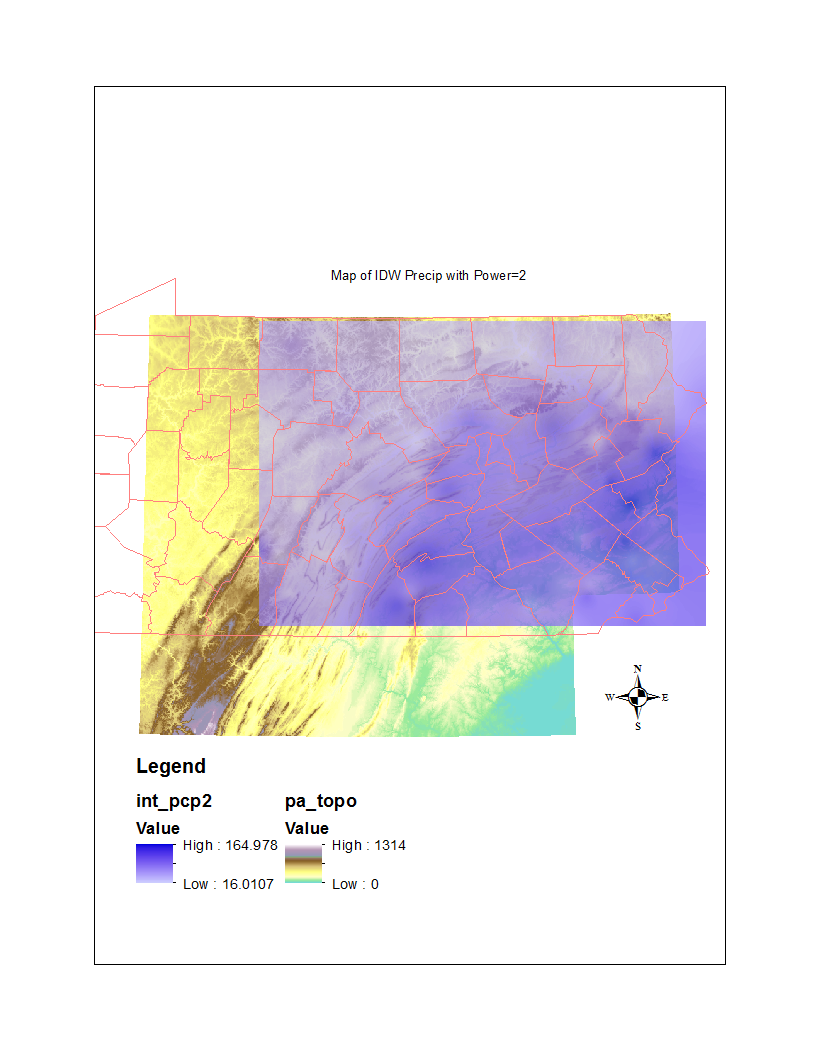
\includegraphics[scale=.9]{./figure/IDWprecip2}
\caption{Map of inverse distance weighting for precipitation with power=2.}
\label{IDWprecip2}
\end{figure}

\begin{figure}
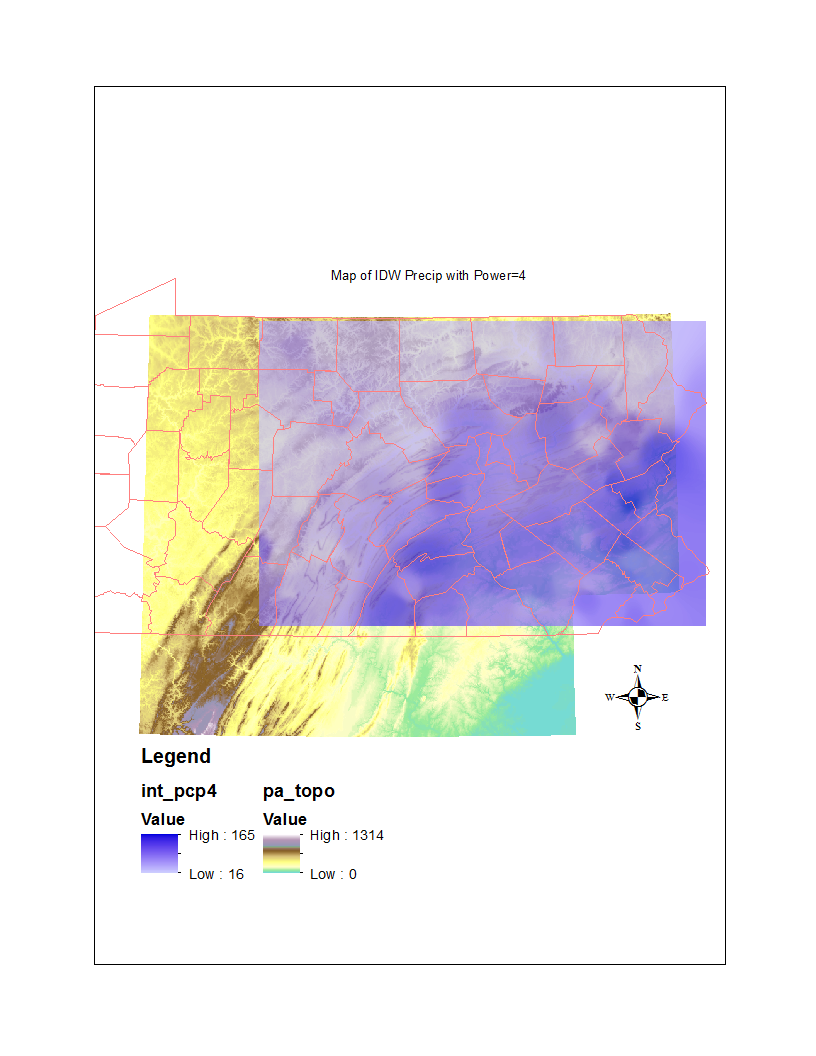
\includegraphics[scale=.9]{./figure/IDWprecip4}
\caption{Map of inverse distance weighting for precipitation with power=4.}
\label{IDWprecip4}
\end{figure}

\begin{figure}
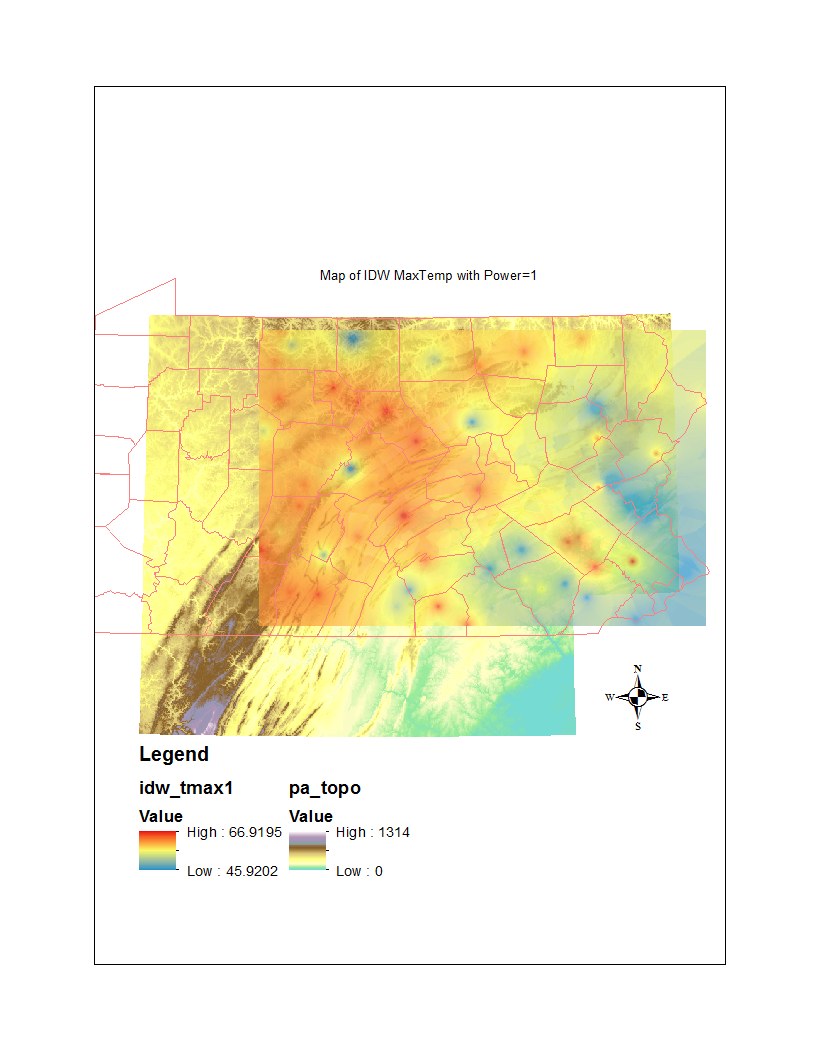
\includegraphics[scale=.9]{./figure/IDWmax1}
\caption{Map of inverse distance weighting for max temperature with power=1}
\label{idwmax1}
\end{figure}

\begin{figure}
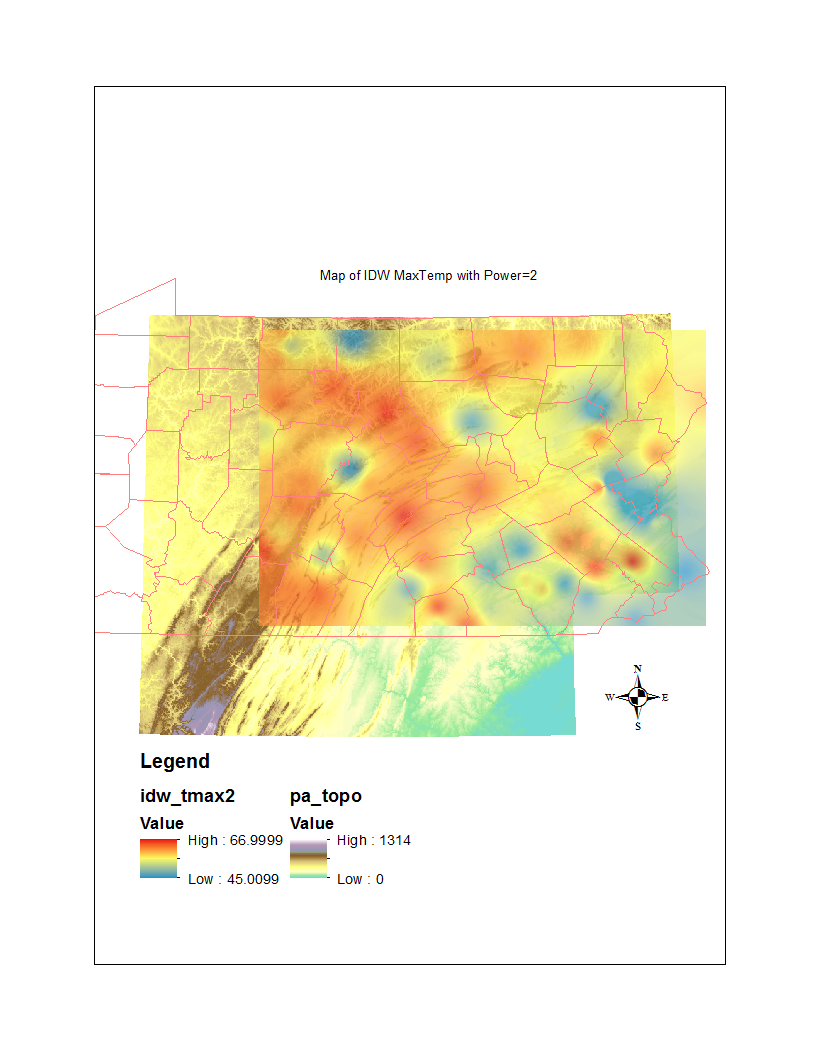
\includegraphics[scale=.9]{./figure/IDWmax2}
\caption{Map of inverse distance weighting for max temperature with power=2}
\label{idwmax2}
\end{figure}

\begin{figure}
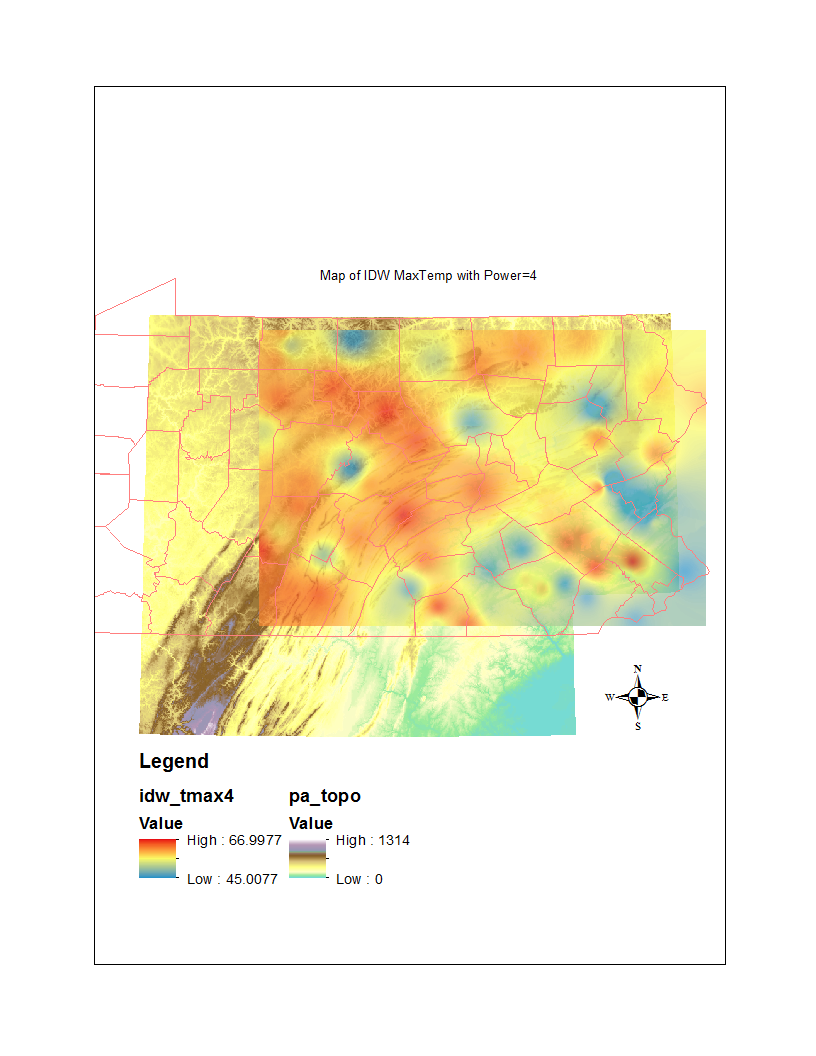
\includegraphics[scale=.9]{./figure/IDWmax4}
\caption{Map of inverse distance weighting for max temperature with power=4}
\label{idwmax4}
\end{figure}

\begin{figure}
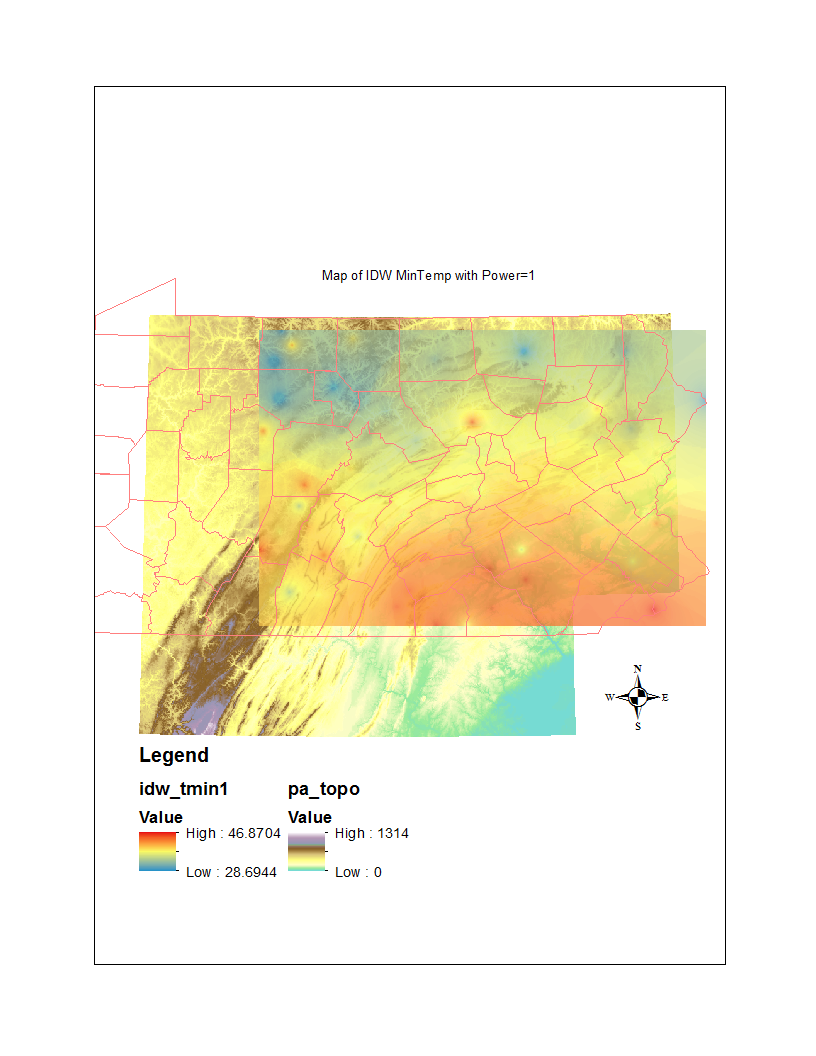
\includegraphics[scale=.9]{./figure/IDWmin1}
\caption{Map of inverse distance weighting for min temperature with power=1}
\label{idwmin1}
\end{figure}

\begin{figure}
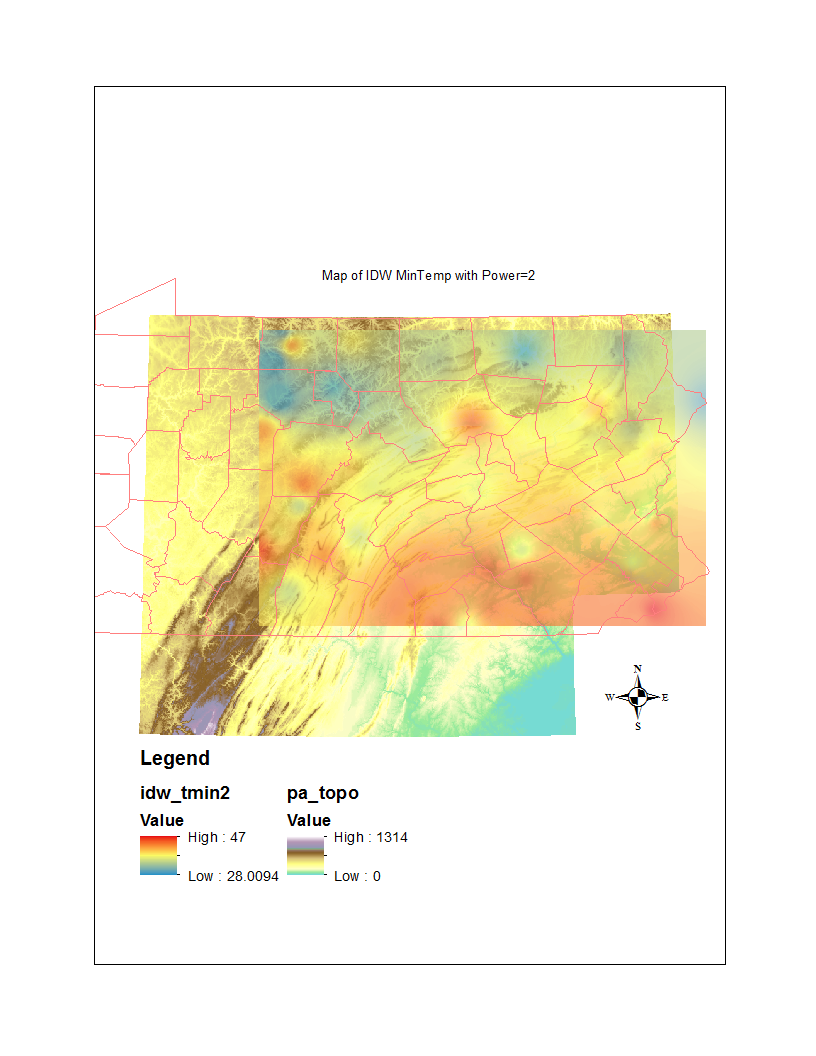
\includegraphics[scale=.9]{./figure/IDWmin2}
\caption{Map of inverse distance weighting for min temperature with power=2}
\label{idwmin2}
\end{figure}

\begin{figure}
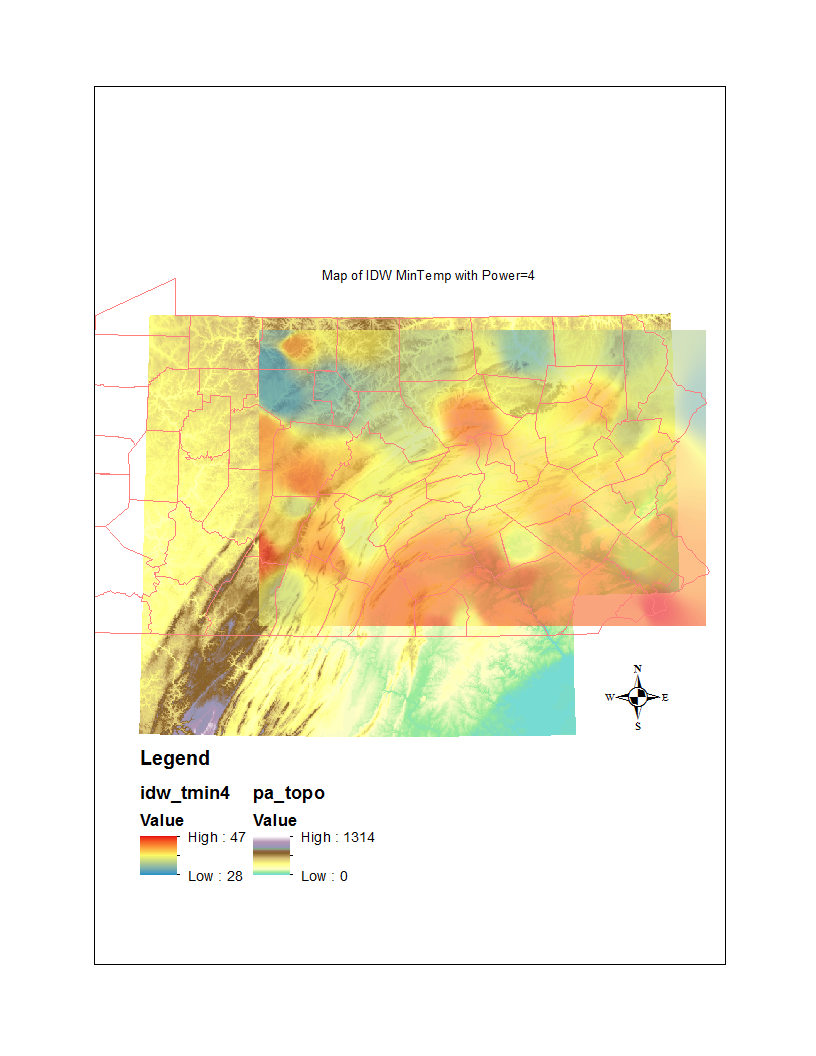
\includegraphics[scale=.9]{./figure/IDWmin4}
\caption{Map of inverse distance weighting for min temperature with power=4}
\label{idwmin4}
\end{figure}

\FloatBarrier


\section{Assignment III: Spline Analysis}
The spline interpolation did not appear to elucidate the trends in precipitation and temperature as well as inverse distance weighting with a small power.  The interpolation appeared to be more patchy and locally fit (figs. ~\ref{spcp}-\ref{smin}).\\

\begin{figure}
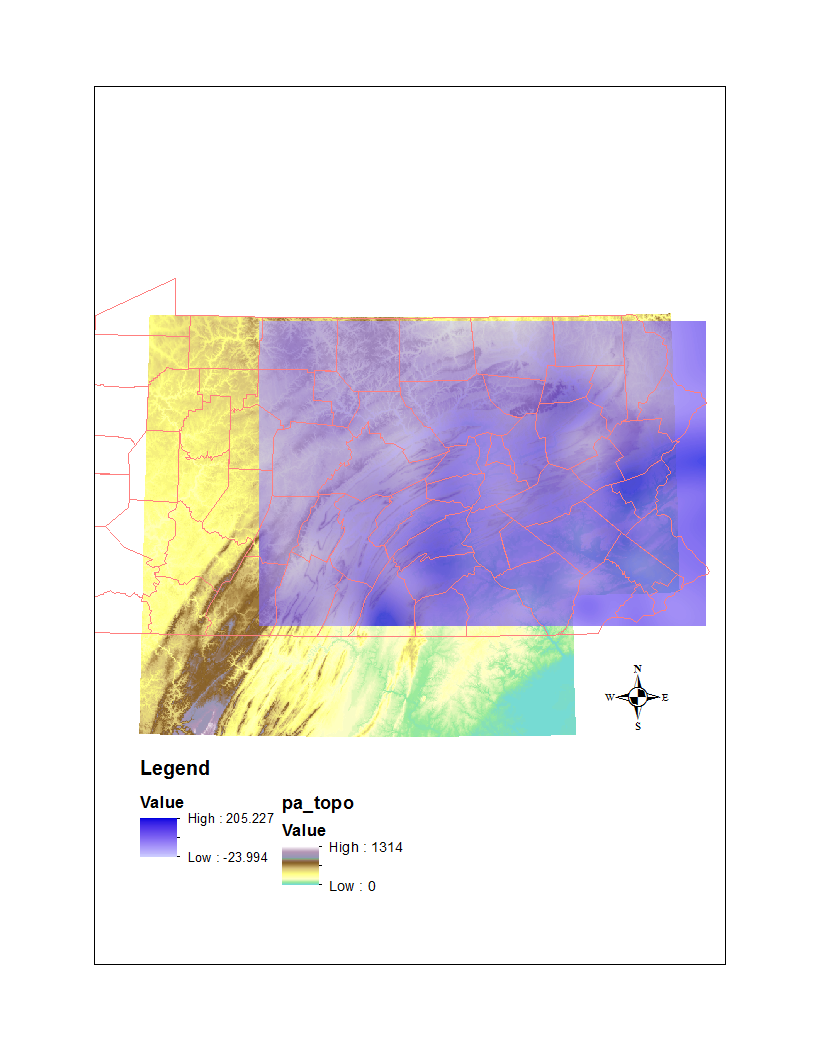
\includegraphics[scale=.9]{./figure/Spline_pcp}
\caption{Map of spline interpolation for precipitation.}
\label{spcp}
\end{figure}

\begin{figure}
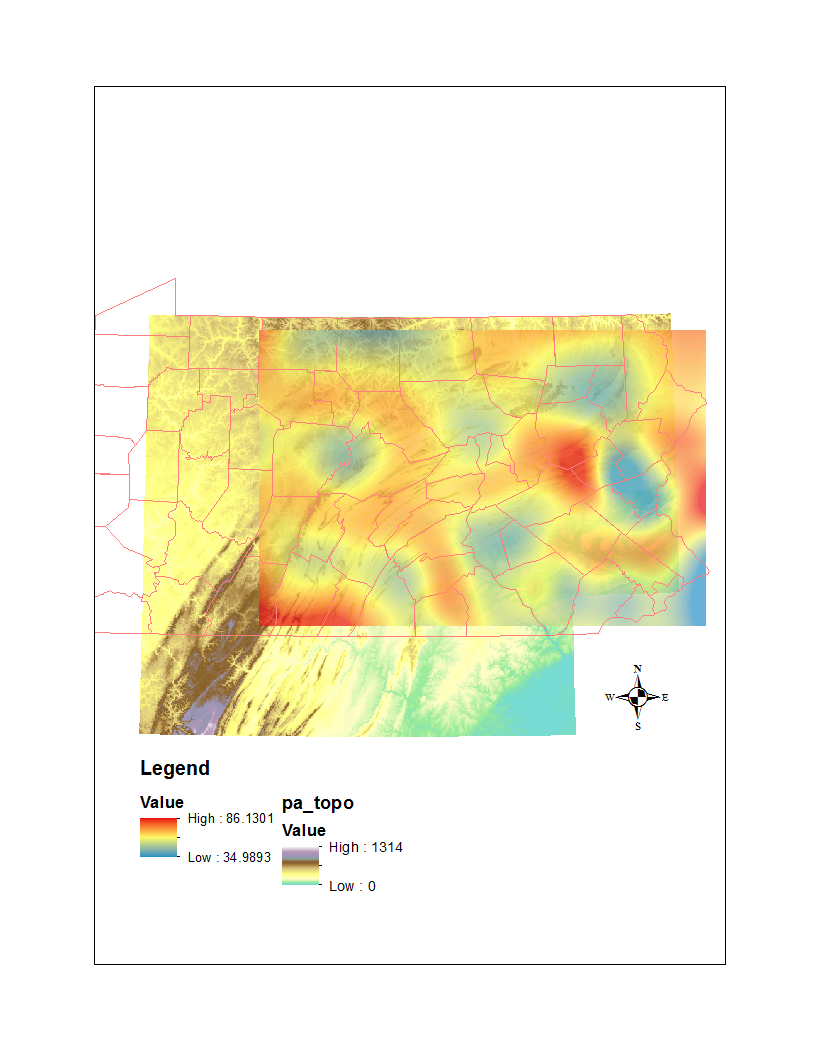
\includegraphics[scale=.9]{./figure/Spline_tmax}
\caption{Map of spline interpolation for max temperature.}
\label{smax}
\end{figure}

\begin{figure}
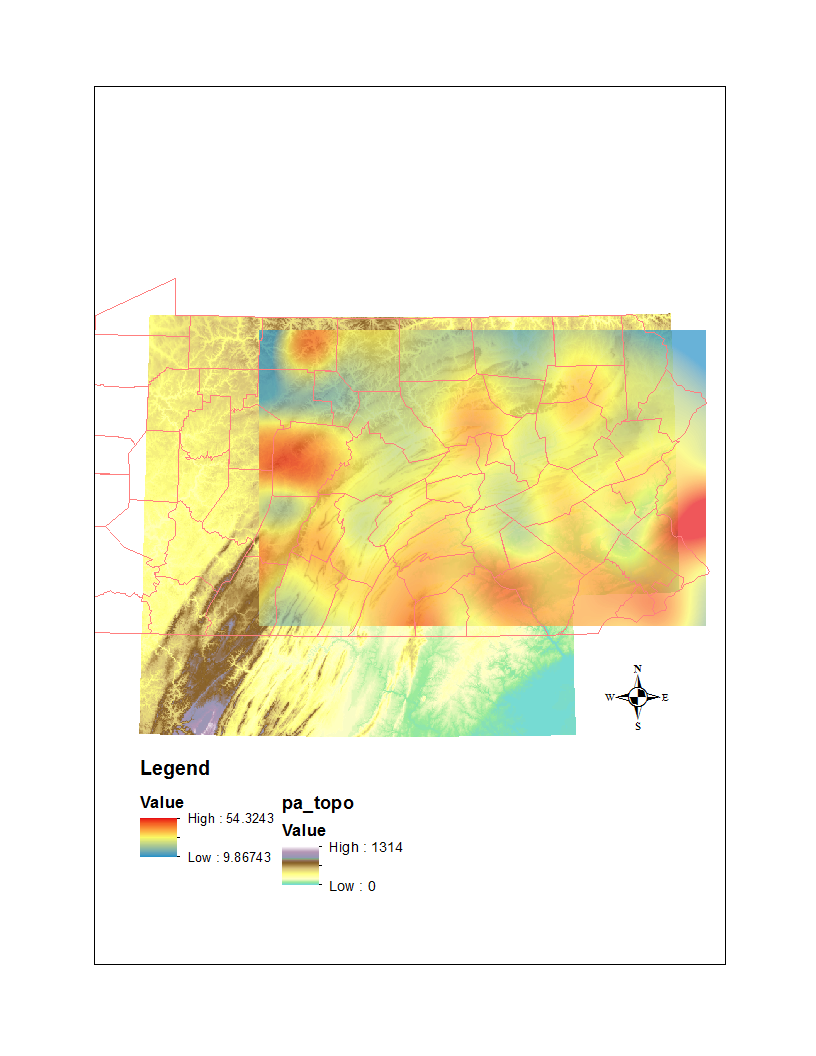
\includegraphics[scale=.9]{./figure/Spline_tmin}
\caption{Map of slpine interpolation for min temperature.}
\label{smin}
\end{figure}

\FloatBarrier

\section{Assigment IV: Trend Analysis}

There does appear to be a trend in precipitation according to the trend analysis (figure~\ref{trend}).  It appears as though there is more precipitation in the lowland areas than in the higher regions.  Interestingly, this is the opposite trend one would expect from orographic weather.\\

\begin{figure}
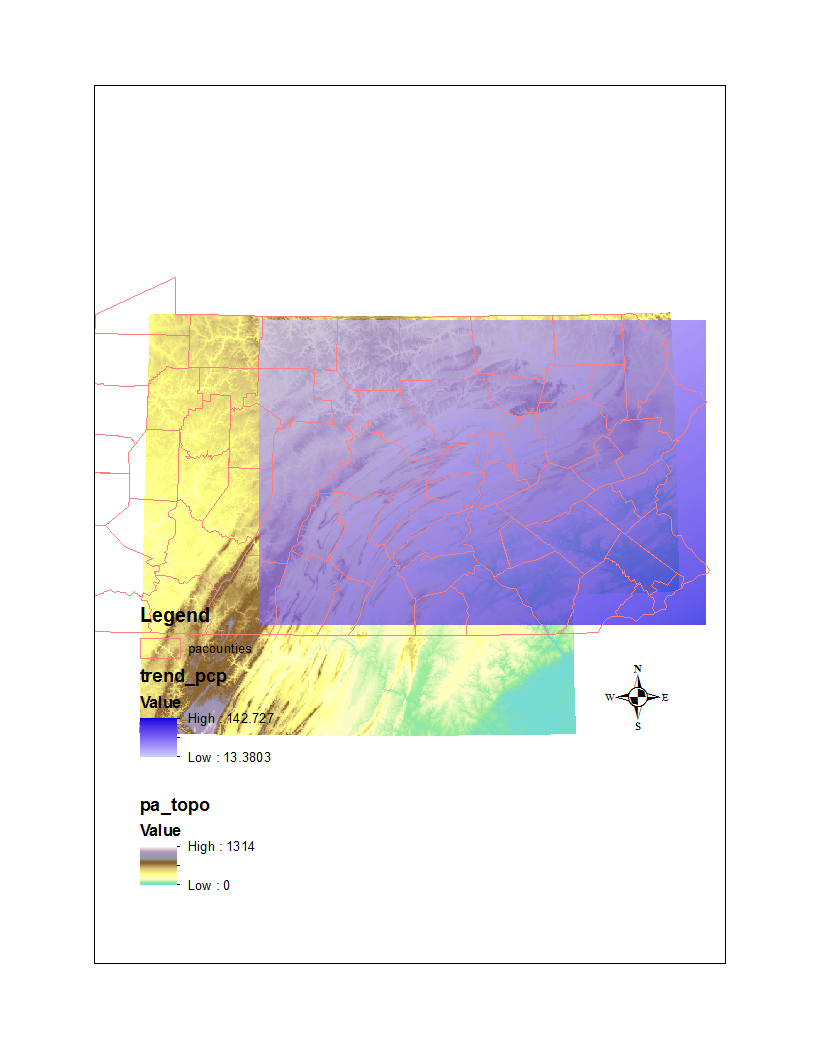
\includegraphics[scale=.9]{./figure/Trend_pcp}
\caption{Map of the trend in precipitation.}
\label{trend}
\end{figure}


\end{document}
